%!TEX root = ../thesis.tex

\section{Benchmarks for self-supervised learning}
\label{section:benchmark}

The previous sections presented various methodologies by which to learn speech
representations from unlabeled corpora. This section surveys the datasets
available to learn and evaluate these representations. We also summarize
several studies and their results to demonstrate the usefulness of the learned
representations for various downstream tasks. 

\subsection{Datasets only for pre-training} 
\Cref{table:datasets} summarizes datasets used for pre-training SSL techniques
in the literature. These datasets are usually large but with limited or no
labels. Libri-light (LL)~\cite{kahn_libri-light_2020}, one of these datasets, is
derived from audiobooks that are part of the
LibriVox\footnote{https://librivox.org/ \label{librivox}} project. LL contains
60k hours of spoken English audio tagged with SNR, speaker ID, and genre
descriptions. The speech examples in Audioset~\cite{gemmeke_audio_2017}, which
consists of over 2M 10-second YouTube video clips human-annotated with 632
audio events, have also been used for pre-training. Audioset has 2.5k hours
of audio of varying quality, different languages, and sometimes multiple sound
sources. AVSpeech~\cite{ephrat_looking_2018} is another large-scale audio-visual
dataset used in SSL research, comprising 4.7k hours of clips from a wide
variety of languages. 
Each clip contains a visible face and audible sound originating from a single
speaker without interfering background signals. The 3100-hour audio part of
AVSpeech has been used to learn audio-only 
representations~\cite{kawakami_learning_2020}. The Fisher corpus~\cite{cieri_fisher_2004} collects
over 2k hours of conversational telephone speech, 1k hours of which is utilized
for pre-training~\cite{jiang_further_2021}. Industrial researchers have also
begun to build large-scale datasets for learning speech representations.
For instance, 10k hours of real-world far-field English voice commands for
self-supervised pre-training have been collected at 
Amazon~\cite{sadhu_wav2vecc_2021}. 

In addition to these English and multilingual efforts, researchers have also
collected corpora for pre-training Chinese speech representations. Didi Dictation
and Didi Callcenter~\cite{jiang_improving_2019, jiang_further_2021} are two
internal datasets containing respectively 10k hours of read speech collected
from mobile dictation application and 10k hours of spontaneous phone calls
between users and customer service staff.

\subsection{Datasets for both pre-training and evaluation}\label{sec:datasets}
Several datasets that provide both speech and associated transcripts and
speaker labels have also been used to develop SSL techniques by enabling
in-domain pre-training and evaluation. Such datasets are also listed in
\cref{table:datasets}. One of the most commonly used datasets in this category
is LibriSpeech (LS)~\cite{panayotov_librispeech_2015}, a labeled corpus
containing 960 hours of
read English speech, which is also derived from an open-source audiobooks
project.\textsuperscript{\ref{librivox}} The corpus consists of subsets
\textit{train-clean-100}, \textit{train-clean-360}, \textit{train-other-500},
\textit{dev-clean}, \textit{dev-other}, \textit{test-clean}, and
\textit{test-other} used for training, development, and testing, respectively.
Subsets tagged with \textit{other} are more challenging utterances from
speakers that yield higher WER as measured with previously built models. LS is
used for unsupervised representation pre-training by ignoring its labels, and
can also be utilized to evaluate the performance of representation on ASR, phoneme recognition (PR),
phoneme classification (PC), and speaker identification (SID) tasks. Wall Street Journal (WSJ)~\cite{paul_design_1992} is another
widely adopted, labeled corpus for pre-training. Its labels can evaluate
performance for ASR, PR, PC, and SID. The original WSJ corpus contains 400 hours
of English read speech data, and today its \textit{si284} (81 hours),
\textit{dev93}, \textit{eval92} subsets are the most-used partitions for
unsupervised training, development, and test, respectively.  The \textit{si84}
(15 hours) partition is also used for training.

The speech community also utilizes multilingual corpora. These are often
large-scale, which facilitates pre-training, but are also partially labeled for ASR
evaluation (PC and PR can be enabled via phone-level forced alignment). These
corpora include Common Voice (CV)~\cite{ardila_common_2020}, Multilingual
LibriSpeech (MLS)~\cite{pratap_mls_2020}, VoxPopuli 
(VP)~\cite{wang_voxpopuli_2021}, and BABEL (BBL)~\cite{gales_speech_2014}. CV is
an open-source, multi-language, growing dataset of voices containing 11k hours
of audio from 76 languages as of the date this review was written (Common Voice
corpus~7.0). Researchers usually use part of this for pre-training (e.g., 7k
hours/60 languages in \cite{babu_xlsr_2021} and 430 hours/29 languages in
\cite{kawakami_learning_2020}) or evaluation. 
MLS derives content from read audiobooks of LibriVox and contains data in eight
European languages for a total of 50k hours of audio. VP comprises a total of 400k
hours of parliamentary speech from the European parliament in 23 European
languages.
The entire dataset~\cite{babu_xlsr_2021} or a 24k-hour 
portion~\cite{chen_unispeechsat_2021, chen_wavlm_2021} thereof has been used for pre-training. BBL
consists of 1k hours of conversational telephone speech in 17 African and Asian
languages.

Several datasets, including GigaSpeech~\cite{chen_gigaspeech_2021}, TED-LIUM~3
(TED3)~\cite{hernandez_tedlium_2018}, TED-LIUM~2 (TED2)~\cite{rousseau_tedlium_2012},
Switchboard (SWB)~\cite{godfrey_switchboard_1992}, 
TIMIT~\cite{garofolo_timit_1993}, and VoxLingua107~\cite{valk_voxlingua107_2021}, are
labeled and conventionally used for evaluation, while their audio streams are
also aggregated to build diversified and large-scale corpora for unsupervised
pre-training~\cite{kawakami_learning_2020, song_speechxlnet_2020, babu_xlsr_2021}.
GigaSpeech is a multi-domain English ASR corpus with 33k hours of audio
collected from audiobooks, podcasts, and YouTube. A subset of 10k audio is
transcribed. TED2 comes with 118 hours of English speech extracted from
TED conference talks and its transcription for evaluating ASR. Its recordings
are clear but with some reverberation. TED3 is an extension of TED2 and
comprises 450 hours of talks. SWB is a 260-hour conversational speech
recognition dataset containing two-sided telephone conversations.
The TIMIT corpus was designed to provide read speech data and its word and
phone-level transcriptions for acoustic-phonetic studies. It contains recordings
in American English. Compared to the previous corpora labeled for ASR
evaluation, VoxLingua107 consists of 6.6k hours of audio in 107 languages and
is annotated for language identification. Beyond the original purpose of
evaluation, these corpora are also used in pre-training to improve the
generalizability of learned representations.

For the purpose of pre-training and evaluating Mandarin speech representations,
the authors of \cite{jiang_improving_2019, jiang_further_2021} also compiled Open Mandarin, 
an open-source Mandarin dataset of 1.5k hours of speech from
the Linguistic Data Consortium (LDC) and
OpenSLR.\footnote{\url{https://openslr.org}} Open Mandarin consists of the HKUST
Mandarin Telephone Speech Corpus (HKUST, 200 hours of spontaneous 
speech, of which
168 hours of audio is used for pre-training; the development and test sets are
excluded.)~\cite{liu_hkust_2006}, AISHELL-1~\cite{bu_aishell1_2017} (178 hours of
read speech),
aidatatang 200zh (200 hours, read speech)~\cite{beijingdatatangtechnologycoltd_aidatatang_}, MAGICDATA
Mandarin Chinese Read Speech Corpus (755 hours, read speech)~\cite{magicdatatechnologycoltd_magicdata_2019},
Free ST Chinese Mandarin Corpus (ST-CMDS, 100 hours, read speech)~\cite{surfingtechcoltd_stcmds_},
and Primewords Chinese Corpus Set 1 (100 hours, read speech)~\cite{primewordsinformationtechnologycoltd_primewords_2018}. 
Both HKUST and AISHELL-1 are labeled and are suitable for ASR evaluation.


\subsection{Datasets for evaluation}

Besides the aforementioned datasets, conventional speech processing benchmarks
are also used to evaluate self-supervised representations. Studies leverage Hub5,
DIRHA, and CHiME-5 to measure the efficacy of representations in ASR.
The Hub5 evaluation (LDC2002T43 and LDC2002S09, also referred to as the NIST 2000
Hub5 English evaluation set) contains 40 transcribed English telephone
conversations only for testing, where 20 are from conversations collected in
SWB studies but not released with the SWB dataset, and the rest are from CallHome
American English Speech (LDC97S42). DIRHA~\cite{ravanelli_dirhaenglish_2015}, short for
Distant-speech Interaction for Robust Home Applications, is a database composed
of utterances sampled from WSJ, speech of keywords and commands, and
phonetically-rich sentences. These utterances are read by UK and US English
speakers and recorded with microphone arrays. CHiME-5~\cite{barker_fifth_2018} is
a challenge that aims to advance robust ASR and presents a dataset of natural
conversational speech collected under a dinner party scenario with microphone
arrays. A team at Amazon Alexa also recorded and transcribed a corpus of 1k
hours of audio for model training and evaluation~\cite{sadhu_wav2vecc_2021}.

Researchers also evaluate representations for sentiment analysis with the
INTERFACE~\cite{hozjan_interface_2002} and MOSEI (CMU Multimodal Opinion
Sentiment and Emotion Intensity)~\cite{zadeh_multimodal_2018} datasets. INTERFACE
is an emotional speech database for Slovenian, English, Spanish, and French,
and contains six emotions: anger, sadness, joy, fear, disgust, and
surprise, plus neutral. MOSEI is comprised of sentence-level sentiment
annotations of 65 hours of YouTube videos
using emotion categories similar to INTERFACE, but replacing joy with
happiness.

In addition, datasets employed to demonstrate the benefit of SSL
representations on various tasks include VCTK \cite{veaux_cstr_2016} and VoxCeleb1 \cite{nagrani_voxceleb_2017} for SID/ASV (automatic speaker verification) tasks, FSC (Fluent Speech Commands) \cite{lugosch_speech_2019} for IC (intent classification), QUESST
(QUESST 2014) \cite{anguera_quesst2014_2015} for QbE (query by example), LS En-Fr \cite{kocabiyikoglu_augmenting_2018} and CoVoST-2 \cite{wang_covost_2020} for ST (speech translation), and ALFFA and OpenSLR-multi for multilingual ASR. The VCTK corpus includes speech
data with 109 English speakers of various accents, each reading out about 400
sentences sampled from newspapers. VoxCeleb1 is an audio-visual dataset
comprised of short YouTube clips containing human speech. It consists of 1251
unique speakers and 352 hours of audio. FSC contains utterances of spoken
English commands that one might use for a smart home or virtual assistant, and
is used to evaluate the performance of a spoken language understanding system.
The QUESST search dataset comprises spoken documents and queries in 6~languages
to measure the capability of models in spotting spoken keywords from documents.
LS En-Fr is a dataset augmenting existing LS monolingual utterances with
corresponding French translations to train and evaluate English-French machine
translators. CoVoST-2 is a multilingual speech translation benchmark based on
CV. It provides data for translating from English into 15 languages and from 21
languages into English, and has a total of 2.9k hours of speech. The ALFFA
project\footnote{\url{http://alffa.imag.fr}} collects speech of African
languages to promote the development of speech technologies in Africa, and
\cite{kawakami_learning_2020} leverages four African languages collected in the
project for evaluation: Amharic~\cite{tachbelie_using_2014}, Fongbe~\cite{laleye_first_2016},
Swahili~\cite{gelas_developments_2012}, and Wolof~\cite{gauthier_collecting_2016}.
In the same work~\cite{kawakami_learning_2020}, the authors
further select 21 phonetically diverse languages from OpenSLR to evaluate the
generalizability of SSL representations across languages. We denote the
collection as OpenSLR-multi below.

Last, \cite{tagliasacchi_pretraining_2020} puts together five datasets 
(MUSAN~\cite{snyder_musan_2015}, Bird Audio Detection~\cite{stowell_automatic_2019},
Speech Commands~\cite{warden_speech_2018}, Spoken Language 
Identification~\cite{oponowicz_spoken_2018}, and TUT Urban Acoustic Scenes 2018~\cite{mesaros_detection_2018}) plus
an SID task built with the LS \textit{train-clean-100} subset to evaluate the
capability of representations on audio event detection.
\cite{quitry_learning_2019} employs the NSynth dataset~\cite{engel_neural_2017} on top
of the six for benchmarking. As many of the datasets are built for research in
audio processing, we here provide only a list of these datasets for reference.



\begin{table*}[ht]
  \centering
  \scriptsize %footnotesize %small, scriptsize, tiny
  \caption[Summary of datasets used for pre-training or evaluation of SSL techniques in the literature.]%
  {Summary of datasets used for pre-training (denoted as PT) or
  evaluation (denoted as EV) of SSL techniques in the literature. The languages and
  sizes of the datasets are provided in columns 3 and 4. Column 5 lists the tasks each
  dataset is used to evaluate. We use the following abbreviations:
  \textbf{EN}: English; 
  \textbf{Multi}: multilingual;
  \textbf{ZH}: Chinese;
  \textbf{Fr}: French; \textbf{ASR}: automatic speech recognition; \textbf{PR}:
  phoneme recognition; \textbf{PC}: phoneme classification; \textbf{SID}:
  speaker identification; \textbf{ASV}: automatic speaker verification;
  \textbf{Sentiment}: sentiment analysis; \textbf{ST}: speech translation;
  \textbf{QbE}: query by example or spoken term detection; \textbf{IC}: intent
  classification; \textbf{AED}: audio event detection; and \textbf{LID}: language
  identification. We distinguish \textbf{PR} from \textbf{PC} based on whether
  the inference is made at the phone level sequentially or the frame level separately.
  \textbf{SID} and \textbf{ASV} both evaluate model capability in encoding
  speaker information; \textbf{SID} classifies one utterance into a pre-defined
  set of speaker labels, whereas \textbf{ASV} infers whether a given pair of
  utterances was uttered by the same speaker.}
  \label{table:datasets}
  \resizebox*{0.99\textwidth}{!}{%
  {\renewcommand*\arraystretch{1.2}
  \begin{tabular}{llllll}
    \toprule
    Dataset & Purpose & Lang. & Size [hours] & Task & License \\
    \midrule
    LibriLight (LL) & PT & EN & 60k & - & MIT License \\ \hline
    AudioSet & PT & Multi & 2.5k & - & CC BY 4.0 \\ \hline %Bidir-CPC, Audio2Vec
    AVSpeech & PT & Multi & 3.1k & - & CC BY 4.0 \\ \hline %Bidir-CPC
    Fisher & PT & EN & 2k/1k \cite{jiang_further_2021}  & - & Linguistic Data Consortium (LDC) \\ \hline % MPC

    Alexa-10k & PT & EN & 10k & - & Not released \\ \hline % wav2vec-c
    Didi Callcenter & PT & ZH & 10k & - & Not released \\ \hline % MPC
    Didi Dictation & PT & ZH & 10k & - & Not released \\ \hline % MPC

    LibriSpeech (LS) & PT/EV & EN & 960 & ASR/PR/PC/SID & CC BY 4.0 \\ \hline
    Wall Street Journal (WSJ) & PT/EV & EN & 81 & ASR/PR/PC/SID & Linguistic Data Consortium (LDC)  \\ \hline

    Common Voice (CV-dataset) & PT/EV & Multi & 11k/7k \cite{babu_xlsr_2021}/430 \cite{kawakami_learning_2020} & ASR/PR/PC & CC0 \\ \hline % mention the split, CPC-modified, Bidir-CPC
    Multilingual LS (MLS) & PT/EV & Multi & 50k & ASR & CC BY 4.0 \\ \hline
    VoxPopuli (VP) & PT/EV & Multi & 400k \cite{babu_xlsr_2021}/24k \cite{chen_unispeechsat_2021, chen_wavlm_2021} & ASR & CC0 \\ \hline
    BABEL (BBL) & PT/EV & Multi & 1k & ASR & IARPA Babel Agreement  \\ \hline

    GigaSpeech & PT/EV & EN & 40k/10k \cite{chen_unispeechsat_2021, chen_wavlm_2021} & ASR & Apache-2.0 License \\ \hline
    TED-LIUM 3 (TED3) & PT/EV & EN & 450 & ASR & CC BY-NC-ND 3.0 \\ \hline %Bidir-CPC
    TED-LIUM 2 (TED2) & PT/EV & EN & 118 & ASR & CC BY-NC-ND 3.0  \\ \hline % speech-XLNet
    Switchboard (SWB) & PT/EV & EN & 260 & ASR & Linguistic Data Consortium (LDC) \\ \hline % MPC, Bidir-CPC
    TIMIT & PT/EV & EN & 4 & ASR/PR/PC & Linguistic Data Consortium (LDC) \\ \hline
    VoxLingua107 & PT/EV & Multi & 6.6k & LID & CC BY 4.0 \\ \hline

    Open Mandarin & PT/EV & ZH & 1.5k & ASR & \makecell[l]{CC BY-NC-ND 4.0, Apache License v.2.0,\\ Linguistic Data Consortium (LDC)} \\ \hline % MPC
    HKUST & PT/EV & ZH & 168/200 & ASR & Linguistic Data Consortium (LDC) \\ \hline % MPC
    AISHELL-1 & PT/EV & ZH & 178 & ASR & Apache License v.2.0 \\ \hline % MPC
    Hub5'00 & EV & EN & 13 & ASR & Linguistic Data Consortium (LDC) \\ \hline % MPC - https://arxiv.org/pdf/1801.00059.pdf
    DIRHA & EV & EN & 11 & ASR & See link for details\textsuperscript{\ref{footnote:DIRHA_license}} \\ \hline % PASE
    CHiME-5 & EV & EN & 50 & ASR & See link for details\textsuperscript{\ref{footnote:CHiME_license}}\\ \hline % PASE+
    Alexa-eval & EV & EN & 1k & ASR & Not released \\ \hline % wav2vec-c
    INTERFACE & EV & Multi & 16 & Sentiment & No information \\ \hline % PASE
    MOSEI & EV & EN & 65 & Sentiment & See link for details\textsuperscript{\ref{footnote:MOSEI_license}}\\ \hline % MockingJay
    VCTK & EV & EN & 44 & SID/ASV & CC BY 4.0 \\ \hline % PASE
    VoxCeleb1 & EV & Multi & 352 & SID/ASV & CC BY 4.0 \\ \hline
    Fluent Speech Commands (FSC) & EV & EN & 14.7 & IC & CC BY-NC-ND 4.0 \\ \hline
    QUESST 2014 (QUESST) & EV & Multi & 23 & QbE & No information \\ \hline
    LS En-Fr & EV & En-Fr & 236 & ST & CC BY 4.0 \\ \hline % APC (tera-9), https://github.com/alicank/Translation-Augmented-LibriSpeech-Corpus
    CoVoST-2 & EV & Multi & 2.9k & ST & CC0 \\ \hline

    ALFFA & EV & Multi & 5.2--18.3 & ASR-multi & MIT License \\ \hline %Bidir-CPC
    OpenSLR-multi & EV & Multi & 4.4--265.9 & ASR-multi & \makecell[l]{CC BY-SA 3.0 US, CC BY-SA 4.0, CC BY 4.0, \\ CC BY-NC-ND 4.0, Apache License v.2.0}\\ \hline %Bidir-CPC
    AED datasets & EV & - & - & AED & \makecell[l]{CC BY 4.0 (MUSAN, Speech Commands, NSynth, Bird Audio\\ Detection),  CC0 (Spoken Language Identification),\\ Non-Commercial (TUT)} \\
    \bottomrule
  \end{tabular}}}
\end{table*}

\addtocounter{footnote}{1}
\footnotetext{\label{footnote:DIRHA_license}\url{https://dirha.fbk.eu/node/107}}
\addtocounter{footnote}{1}
\footnotetext{\label{footnote:CHiME_license}\url{https://chimechallenge.github.io/chime6/download.html}}
\addtocounter{footnote}{1}
\footnotetext{\label{footnote:MOSEI_license}\url{https://github.com/A2Zadeh/CMU-MultimodalSDK/blob/master/LICENSE.txt}}

\begin{table*}[ht]
  \centering
  \tiny
  \caption[Summary of common experiment settings for various SSL
  evaluations (Part 1).]{A summary of common experiment settings for various SSL
  evaluations (Part 1). Networks are usually pre-trained with SSL
  techniques, augmented with prediction heads, and fine-tuned (or trained) with
  labeled data in downstream tasks for benchmarking. The 
  \textbf{Pre-training corpus}, \textbf{Training (fine-tuning)}, and
  \textbf{Test} columns list the datasets used in each work, and the \textbf{Task}
  column lists the tasks performed in the corresponding papers. We follow
  the abbreviation introduced in \cref{table:datasets}. The \textbf{Transfer}
  column indicates whether the SSL technique is evaluated by its capability for
  transfer learning, i.e., different datasets are utilized for pre-training and
  fine-tuning. The \textbf{Fine-tuning labels used} column summarizes the
  amount of labeled examples used in downstream fine-tuning.}
  \label{table:method_data_setting}
  \resizebox*{0.97\textwidth}{!}{%
  {%\tabulinesep=1mm
  \renewcommand*\arraystretch{1.4}
  \begin{tabular}{p{0.12\textwidth}p{0.12\textwidth}p{0.06\textwidth}p{0.13\textwidth}p{0.13\textwidth}p{0.06\textwidth}p{0.20\textwidth}}
    \toprule
    \multirow{2}{*}{Work} & \multirow{2}{*}{\makecell[l]{Pre-training\\ corpus}} & \multirow{2}{*}{Task} & \multicolumn{2}{c}{Dataset} & \multirow{2}{*}{Transfer} & \multirow{2}{*}{Fine-tuning labels used} \\ \cline{4-5}
     &  &  & Training (fine-tuning) & Test & & \\
    \midrule
    % CPC
    \multirow{2}{*}[0mm]{CPC \cite{oord_representation_2018}} & \multirow{2}{*}[0mm]{LS 100 hrs} & PC & LS 100 hrs\textsuperscript{\ref{footnote:CPC-split}} & LS 100 hrs\textsuperscript{\ref{footnote:CPC-split}} & - & 80\textsuperscript{\ref{footnote:low-resource}} hrs \\ \cline{3-7}
    & & SID & LS 100 hrs\textsuperscript{\ref{footnote:CPC-split}} & LS 100 hrs\textsuperscript{\ref{footnote:CPC-split}} & - & 80\textsuperscript{\ref{footnote:low-resource}} hrs \\ \hline
    % PASE
    \multirow{2}{*}[-5mm]{PASE\cite{pascual_learning_2019}} & \multirow{2}{*}[-5mm]{LS 50 hrs \cite{ravanelli_learning_2018}} & SID & VCTK\textsuperscript{\ref{footnote:official-split}} & VCTK\textsuperscript{\ref{footnote:official-split}} & \checkmark & 44 hrs \\ \cline{3-7}
    & & Sentiment & INTERFACE\textsuperscript{\ref{footnote:interface-split}} & INTERFACE\textsuperscript{\ref{footnote:interface-split}} & \checkmark & 3 hrs \\ \cline{3-7}
    & & PR & TIMIT\textsuperscript{\ref{footnote:official-split}} & TIMIT\textsuperscript{\ref{footnote:official-split}} & \checkmark & 4 hrs \\ \cline{3-7}
    & & ASR & DIRHA\textsuperscript{\ref{footnote:official-split}} & DIRHA\textsuperscript{\ref{footnote:official-split}} & \checkmark & 11 hrs \\ \hline
    % Audio2Vec
    Audio2Vec \cite{tagliasacchi_pretraining_2020} & AudioSet & AED & 6 AED datasets\textsuperscript{\ref{footnote:AED-datasets}} & 6 AED datasets\textsuperscript{\ref{footnote:AED-datasets}} & \checkmark & See \cite{tagliasacchi_pretraining_2020} for details \\ \hline
    % APC
    \multirow{3}{*}[0mm]{APC \cite{chung_unsupervised_2019, chung_generative_2020}} & \multirow{3}{*}[0mm]{LS 360 hrs} & ASR & WSJ si284\textsuperscript{\ref{footnote:91-split-dev}} & WSJ dev93 & \checkmark & 72 hrs \\ \cline{3-7}
    & & ST & LS En-Fr\textsuperscript{\ref{footnote:official-split}} & LS En-Fr\textsuperscript{\ref{footnote:official-split}} & - & 236 hrs \\ \cline{3-7}
    & & SID & WSJ si284\textsuperscript{\ref{footnote:APC-split}} & WSJ si284\textsuperscript{\ref{footnote:APC-split}} & \checkmark & 65\textsuperscript{\ref{footnote:low-resource}} hrs \\ \hline
    % wav2vec
    \multirow{2}{*}[0mm]{wav2vec \cite{schneider_wav2vec_2019}} & \multirow{2}{*}[-0.5mm]{\makecell[l]{LS 80/960 hrs,\\ LS 960 hrs \\ \:+ WSJ si284}} & ASR & WSJ si284 & WSJ eval92 & \checkmark & 81 hrs\vspace{1mm} \\ \cline{3-7}
    & & PR & TIMIT\textsuperscript{\ref{footnote:official-split}} & TIMIT\textsuperscript{\ref{footnote:official-split}} & \checkmark & 4 hr\vspace{1mm} \\ \hline
    % Phase predict
    PhasePredict \cite{quitry_learning_2019} & AudioSet & AED & 7 AED datasets\textsuperscript{\ref{footnote:AED-datasets}} & 7 AED datasets\textsuperscript{\ref{footnote:AED-datasets}} & \checkmark & See \cite{quitry_learning_2019} for details \\ \hline
    % Bidir-CPC
    \multirow{3}{*}{Bidir-CPC\cite{kawakami_learning_2020}} & \multirow{3}{*}{\makecell[l]{LS 960 hrs,\\ CPC-8k\textsuperscript{\ref{footnote:CPC-8k}}}} & ASR & \makecell[l]{WSJ si284,\\LS 960 hrs,\\TED3\textsuperscript{\ref{footnote:official-split}}} & \makecell[l]{WSJ eval92,\\LS test-clean,\\LS test-other,\\TED3\textsuperscript{\ref{footnote:official-split}}, SWB\textsuperscript{\ref{footnote:official-split}}}  & \makecell[l]{Different\\ datasets for\\ training\\ and test} & 81/960/450 hrs \\ \cline{3-7} % cross domain transferring, SWB eval2000, TED3 training set size = 450 hrs
    & & \makecell[l]{ASR-multi} & ALFFA\textsuperscript{\ref{footnote:official-split}} & ALFFA\textsuperscript{\ref{footnote:official-split}} & \checkmark & 4 languages, 5.2--18.3 hrs\\ \cline{3-7}
    & & \makecell[l]{ASR-multi} & OpenSLR-multi\textsuperscript{\ref{footnote:official-split}} & OpenSLR-multi\textsuperscript{\ref{footnote:official-split}} & \checkmark & 21 languages, 4.4--265.9 hrs \\ \hline
    % vq-VAE
    % MockingJay
    \multirow{3}{*}{MockingJay \cite{liu_mockingjay_2020}} & \multirow{3}{*}{\makecell[l]{LS 360 hrs}} & PC & LS 360 hrs & LS test-clean & - & 0.36\textsuperscript{\ref{footnote:low-resource}} /1.8\textsuperscript{\ref{footnote:low-resource}} /3.6\textsuperscript{\ref{footnote:low-resource}} /18\textsuperscript{\ref{footnote:low-resource}} /45\textsuperscript{\ref{footnote:low-resource}} /360  hrs \\ \cline{3-7}
    & & SID & LS 100 hrs\textsuperscript{\ref{footnote:91-split-test}} & LS 100 hrs\textsuperscript{\ref{footnote:91-split-test}} & - & 90\textsuperscript{\ref{footnote:low-resource}} hrs \\ \cline{3-7}
    & & Sentiment & MOSEI\textsuperscript{\ref{footnote:official-split}} & MOSEI\textsuperscript{\ref{footnote:official-split}} & \checkmark & 65 hrs \\ \hline
    % CPC modified
    \multirow{2}{*}{CPC modified \cite{riviere_unsupervised_2020}} & LS 100 hrs & PC & LS 100 hrs\textsuperscript{\ref{footnote:CPC-split}} & \makecell[l]{LS 100 hrs\textsuperscript{\ref{footnote:CPC-split}}} & - & \makecell[l]{80\textsuperscript{\ref{footnote:low-resource}} hrs} \\ \cline{2-7}
    & \makecell[l]{LS 100 hrs,\\LS 960 hrs,\\LL 60k hrs} & PC & CV-dataset\textsuperscript{\ref{footnote:official-split}} & CV-dataset\textsuperscript{\ref{footnote:official-split}} & \checkmark & 1 hrs \\ \hline
    % vq-wav2vec
    \multirow{2}{*}[0mm]{vq-wav2vec \cite{baevski_vqwav2vec_2020}} & \multirow{2}{*}[0mm]{LS 960 hrs} & ASR & WSJ si284 & \makecell[l]{WSJ eval92} & \checkmark & \makecell[l]{81 hrs} \\ \cline{3-7}
    & & PR & TIMIT\textsuperscript{\ref{footnote:official-split}} & TIMIT\textsuperscript{\ref{footnote:official-split}} & \checkmark & 4 hrs \\ \hline
    % DeCoAR
    \multirow{2}{*}[0mm]{DeCoAR \cite{ling_deep_2020}} & \multirow{2}{*}[0mm]{\makecell[l]{LS 100/360/\\\:\:\:460/960 hrs,\\ WSJ si284}} & ASR & WSJ si284 & WSJ eval92 & - & \makecell[l]{25\textsuperscript{\ref{footnote:low-resource}}/40\textsuperscript{\ref{footnote:low-resource}}/81 hrs} \\ \cline{3-7}
    & & ASR & \makecell[l]{LS 100/360/\\\:\:\:460/960 hrs} & \makecell[l]{LS test-clean,\\ LS test-other} & - & 100/360/460/960 hrs \\ \hline
    % MT-APC
    \multirow{2}{*}[0mm]{MT-APC\cite{chung_improved_2020}} & \multirow{2}{*}[0mm]{LS 360 hrs} & ASR & WSJ si284\textsuperscript{\ref{footnote:91-split-dev}} & WSJ dev93 & \checkmark & 72 hrs \\ \cline{3-7}
    & & ST & LS En-Fr\textsuperscript{\ref{footnote:official-split}} & LS En-Fr\textsuperscript{\ref{footnote:official-split}} & - & 236 hrs \\ \hline
    % PASE+
    \multirow{3}{*}[0mm]{PASE+\cite{ravanelli_multitask_2020}} & \multirow{3}{*}[0mm]{LS 50 hrs \cite{ravanelli_learning_2018}} & PR & TIMIT\textsuperscript{\ref{footnote:official-split}} & TIMIT\textsuperscript{\ref{footnote:official-split}} & \checkmark & 4 hrs \\ \cline{3-7}
    & & ASR & DIRHA\textsuperscript{\ref{footnote:official-split}} & DIRHA\textsuperscript{\ref{footnote:official-split}} & \checkmark & 11 hrs \\ \cline{3-7}
    & & ASR & CHiME-5\textsuperscript{\ref{footnote:official-split}} & CHiME-5\textsuperscript{\ref{footnote:official-split}} & \checkmark & 50 hrs \\ \hline
    % AALBERT
    \multirow{2}{*}[0mm]{AALBERT \cite{chi_audio_2020}} & \multirow{2}{*}[0mm]{\makecell[l]{LS 360 hrs}} & PC & LS 100 hrs\textsuperscript{\ref{footnote:APC-split}} & LS 100 hrs\textsuperscript{\ref{footnote:APC-split}} & - & 80\textsuperscript{\ref{footnote:low-resource}} hrs \\ \cline{3-7}
    & & SID & LS 360 hrs\textsuperscript{\ref{footnote:APC-split}} & LS 360 hrs\textsuperscript{\ref{footnote:APC-split}} & - & 288\textsuperscript{\ref{footnote:low-resource}} hrs \\
    \bottomrule
  \end{tabular}}}
\end{table*}


\begin{table*}[ht]
  \centering
  \tiny
  \caption[Summary of common experiment settings for various SSL
  evaluations (Part 2).]{A summary of common experiment settings for various SSL
  evaluations (Part 2). See the caption of \cref{table:method_data_setting} for a
  detailed description of all the abbreviations used in this table.}
  \label{table:method_data_setting_2}
  \resizebox*{0.97\textwidth}{!}{%
  {%\tabulinesep=1mm
  \renewcommand*\arraystretch{1.4}
  \begin{tabular}{p{0.12\textwidth}p{0.12\textwidth}p{0.05\textwidth}p{0.18\textwidth}p{0.18\textwidth}p{0.05\textwidth}p{0.15\textwidth}}
    \toprule
    \multirow{2}{*}{Work} & \multirow{2}{*}{\makecell[l]{Pre-training\\ corpus}} & \multirow{2}{*}{Task} & \multicolumn{2}{c}{Dataset} & \multirow{2}{*}{Transfer} & \multirow{2}{*}{Fine-tuning labels used} \\ \cline{4-5}
     &  &  & Training (fine-tuning) & Test & & \\
    \midrule
    % BMR
    \multirow{2}{*}[0mm]{BMR \cite{wang_unsupervised_2020}} & \multirow{2}{*}[0mm]{\makecell[l]{WSJ si284,\\LS 960 hrs}} & ASR & WSJ si284 & WSJ eval92 & - & 81 hrs \\ \cline{3-7}
    & & PR & WSJ si84/si284 & WSJ dev93 & - & 15/81 hrs \\ \hline
    % vq-APC
    \multirow{2}{*}[0mm]{vq-APC \cite{chung_vectorquantized_2020}} & \multirow{2}{*}[0mm]{LS 360 hrs} & PC & WSJ si284\textsuperscript{\ref{footnote:91-split-dev}} & \makecell[l]{WSJ dev93} & \checkmark & \makecell[l]{81 hrs} \\ \cline{3-7}
    & & SID & WSJ si284\textsuperscript{\ref{footnote:APC-split}} & WSJ si284\textsuperscript{\ref{footnote:APC-split}} & \checkmark & 65\textsuperscript{\ref{footnote:low-resource}} hrs \\ \hline
    % vq-wav2vec + Discrete BERT
    \makecell[l]{vq-wav2vec + \\DiscreteBERT \cite{baevski_effectiveness_2020}} & LS 960 hrs & ASR & LS 100 hrs & \makecell[l]{LS test-clean,\\ LS test-other} & - & \makecell[l]{10 mins\textsuperscript{\ref{footnote:low-resource}},\\ 1\textsuperscript{\ref{footnote:low-resource}}/10\textsuperscript{\ref{footnote:low-resource}}/100 hrs} \\ \hline
    % speech-XLNet
    \multirow{2}{*}[-1mm]{speech-XLNet \cite{song_speechxlnet_2020}} & \multirow{2}{*}[-1mm]{\makecell[l]{LS 960 hrs\\\;\;\;+ WSJ si284\\\;\;\;+ TED2}} & PR & TIMIT\textsuperscript{\ref{footnote:official-split}} & TIMIT\textsuperscript{\ref{footnote:official-split}} & \checkmark & 4 hrs\vspace{1mm} \\ \cline{3-7}
    & & ASR & WSJ si284 & WSJ eval92 & - & \makecell[l]{7\textsuperscript{\ref{footnote:low-resource}}/14\textsuperscript{\ref{footnote:low-resource}}/30\textsuperscript{\ref{footnote:low-resource}}/81 hrs}\vspace{1mm} \\ \hline
    % MPC
    \multirow{3}{*}[0mm]{MPC \cite{jiang_improving_2019, jiang_further_2021}} & \multirow{2}{*}[0mm]{\makecell[l]{Didi Callcenter,\\Didi Dictation,\\Open Mandarin}} & ASR-zh & HKUST\textsuperscript{\ref{footnote:official-split}} & HKUST\textsuperscript{\ref{footnote:official-split}} & \checkmark & 168 hrs \\ \cline{3-7}
    & & ASR-zh & AISHELL-1\textsuperscript{\ref{footnote:official-split}} & AISHELL-1\textsuperscript{\ref{footnote:official-split}} & \checkmark & 178 hrs\vspace{1mm} \\ \cline{2-7}
    & \multirow{1}{*}[-0.5mm]{\makecell[l]{SWB, Fisher 1k,\\LS 960 hrs}} & ASR & SWB & Hub5'00 & - & 260 hrs \vspace{2.5mm} \\ \hline
    % MPE
    \multirow{2}{*}[0mm]{MPE \cite{liu_masked_2020}} & \multirow{2}{*}[0mm]{\makecell[l]{WSJ si284,\\LS 960 hrs}} & ASR & WSJ si284 & WSJ eval92 & - & \makecell[l]{25\textsuperscript{\ref{footnote:low-resource}}/40\textsuperscript{\ref{footnote:low-resource}}/81 hrs} \\ \cline{3-7}
    & & ASR & LS 100/360/960 hrs & LS test-clean & - & 100/360/960 hrs \\ \hline
    % ConvDMM
    ConvDMM \cite{khurana_convolutional_2020} & \makecell[l]{LS 50\cite{ravanelli_learning_2018}/360/\\\:\:\:960 hrs} & PC/PR & WSJ si284 & WSJ eval92 & \checkmark & \makecell[l]{5\textsuperscript{\ref{footnote:low-resource}}/50\textsuperscript{\ref{footnote:low-resource}}/100\textsuperscript{\ref{footnote:low-resource}} mins,\\ 4\textsuperscript{\ref{footnote:low-resource}}/8\textsuperscript{\ref{footnote:low-resource}}/40\textsuperscript{\ref{footnote:low-resource}} hrs} \\ \hline
    % wav2vec 2.0
    \multirow{2}{*}{wav2vec 2.0 \cite{baevski_wav2vec_2020}} & \multirow{2}{*}{\makecell[l]{LS 960 hrs,\\ LL 60k hrs}} & ASR & LS 960 hrs & \makecell[l]{LS test-clean,\\ LS test-other} & - & \makecell[l]{10 mins\textsuperscript{\ref{footnote:low-resource}},\\ 1\textsuperscript{\ref{footnote:low-resource}}/10\textsuperscript{\ref{footnote:low-resource}}/100/960 hrs} \\ \cline{3-7}
    & & PR & TIMIT\textsuperscript{\ref{footnote:official-split}} & TIMIT\textsuperscript{\ref{footnote:official-split}} & \checkmark & 4 hrs \\ \hline
    % NPC
    \multirow{2}{*}[0mm]{NPC \cite{liu_nonautoregressive_2020}} & \multirow{2}{*}[0mm]{LS 360 hrs} & PC & WSJ si284\textsuperscript{\ref{footnote:91-split-dev}} & \makecell[l]{WSJ dev93} & \checkmark & \makecell[l]{81 hrs} \\ \cline{3-7}
    & & SID & WSJ si284\textsuperscript{\ref{footnote:APC-split}} & WSJ si284\textsuperscript{\ref{footnote:APC-split}} & \checkmark & 65\textsuperscript{\ref{footnote:low-resource}} hrs \\ \hline
    % DeCoAR 2.0
    DeCoAR 2.0 \cite{ling_decoar_2020} & LS 960 hrs & ASR & \makecell[l]{LS 100 hrs} & \makecell[l]{LS test-clean,\\ LS test-other} & - & \makecell[l]{1\textsuperscript{\ref{footnote:low-resource}}/10\textsuperscript{\ref{footnote:low-resource}}/100 hrs} \\ \hline
    % TERA
    \multirow{4}{*}[0mm]{TERA \cite{liu_tera_2021}} & \multirow{4}{*}[0mm]{\makecell[l]{LS 100/360/\\\:\:\:960 hrs}} & PC & LS 100 hrs\textsuperscript{\ref{footnote:CPC-split}} & LS 100 hrs\textsuperscript{\ref{footnote:CPC-split}} & - & 80\textsuperscript{\ref{footnote:low-resource}} hrs \\ \cline{3-7}
    & & SID & LS 100 hrs\textsuperscript{\ref{footnote:CPC-split}} & LS 100 hrs\textsuperscript{\ref{footnote:CPC-split}} & - & 80\textsuperscript{\ref{footnote:low-resource}} hrs \\ \cline{3-7}
    & & PR & TIMIT\textsuperscript{\ref{footnote:official-split}} & TIMIT\textsuperscript{\ref{footnote:official-split}} & \checkmark & 4 hrs \\ \cline{3-7}
    & & ASR & LS 100 hrs & LS test-clean & - & 100 hrs \\ \hline
    % HuBERT
    HuBERT \cite{hsu_hubert_2021} & \makecell[l]{LS 960 hrs,\\ LL 60k hrs} & ASR & LS 960 hrs & \makecell[l]{LS test-clean\\ LS test-other} & - & \makecell[l]{10 mins\textsuperscript{\ref{footnote:low-resource}}, 1\textsuperscript{\ref{footnote:low-resource}}\\/10\textsuperscript{\ref{footnote:low-resource}}/100/960 hrs} \\ \hline
    % wav2vec-c
    wav2vec-c \cite{sadhu_wav2vecc_2021} & Alexa-10k & ASR & \makecell[l]{Alexa-eval} & \makecell[l]{Alexa-eval} & \checkmark & 1k hrs \\ \hline
    UniSpeech-SAT \cite{chen_unispeechsat_2021} & \makecell[l]{LL 60k hrs\\\;\;+ GigaSpeech-10k\\\;\;+ VP-24k} & Multi & SUPERB & SUPERB & \checkmark & See SUPERB \cite{yang_superb_2021} paper for details \\ \hline
    WavLM \cite{chen_wavlm_2021} & \makecell[l]{LL 60k hrs\\\;\;+ GigaSpeech-10k\\\;\;+ VP-24k} & Multi & SUPERB & SUPERB & \checkmark & See \cite{yang_superb_2021} for details \\ \hline
    \multirow{4}{*}[0mm]{XLS-R \cite{babu_xlsr_2021}} & \multirow{4}{*}[0mm]{\makecell[l]{VP-400k + MLS\\\;\;+ CV-dataset-7k\\\;\;+ VL\\\;\;+ BBL}} & ASR & VP, MLS, CV-dataset, BBL, LS & VP, MLS, CV-dataset, BBL, LS & - & \multirow{4}{*}[0mm]{See \cite{babu_xlsr_2021} for details} \\ \cline{3-6}
    & & SID & VoxCeleb1 & VoxCeleb1 & \checkmark & \\ \cline{3-6}
    & & ST & CoVoST-2 & CoVoST-2 & \checkmark & \\ \cline{3-6}
    & & LID & VL & VL & - & \\
    \bottomrule
  \end{tabular}}}
\end{table*}

\addtocounter{footnote}{1}
\footnotetext{\label{footnote:CPC-split}
Train/test split made available
by \cite{oord_representation_2018} on Google drive
https://drive.google.com/drive/folders/1BhJ2umKH3whguxMwifaKtSra0TgAbtfb.}
\addtocounter{footnote}{1}
\footnotetext{\label{footnote:official-split}
Utilizes official training or test split.}

\addtocounter{footnote}{1}
\footnotetext{\label{footnote:interface-split}
English utterances used in experiments. The utterances correspond to
approximately 3~hours for training, 40~minutes for development, and 30~minutes
for testing.}

\addtocounter{footnote}{1}
\footnotetext{\label{footnote:AED-datasets}
The 6 AED datasets used in
\cite{tagliasacchi_pretraining_2020} are MUSAN~\cite{snyder_musan_2015}, Bird Audio
Detection~\cite{stowell_automatic_2019}, Speech Commands~\cite{warden_speech_2018},
Spoken Language Identification~\cite{oponowicz_spoken_2018}, TUT Urban Acoustic
Scenes 2018~\cite{mesaros_detection_2018} plus an SID task built with LS
\textit{train-clean-100}. In addition to the 6 datasets,
\cite{quitry_learning_2019} use the NSynth dataset~\cite{engel_neural_2017} for
evaluation.}
\addtocounter{footnote}{1}
\footnotetext{\label{footnote:CPC-8k}
A collection of AudioSet, AVSpeech,
CV-dataset, LS, WSJ, TIMIT, Speech Accent Archive 
(SSA)~\cite{weinberger_speech_2011}, TED3, and SWB. SSA is a growing annotated corpus of
English speech with various accents. Among the papers studied in this review, SSA
is used in \cite{kawakami_learning_2020} only for pre-training, and only 1 hour
of audio is utilized. Thus, we exclude it from our discussion in
\cref{section:benchmark}.}
\addtocounter{footnote}{1}
\footnotetext{\label{footnote:low-resource}
A subset of the official training
split is sampled, usually to mimic low-resource learning conditions or to
quickly evaluate for training and testing on the same split but disjoint
subsets.}
\addtocounter{footnote}{1}
\footnotetext{\label{footnote:APC-split}
Dataset split into training,
validation, and test subsets at a ratio of 8:1:1.}
\addtocounter{footnote}{1}
\footnotetext{\label{footnote:91-split-dev}
Dataset split into training
and validation subsets at a ratio of 9:1.}
\addtocounter{footnote}{1}
\footnotetext{\label{footnote:91-split-test}
The dataset split into training
and test subsets at a ratio of 9:1.}

\subsection{Experiment settings for evaluating SSL techniques}
A common way to benchmark SSL techniques and show their efficacy is to
fine-tune a pre-trained SSL model for a supervised downstream task.
Depending on the corpora used in pre-training and fine-tuning, techniques can
be benchmarked in terms of their capability to transfer knowledge across datasets
(i.e., using pre-training corpora that differ from the fine-tuning ones), their
benefit when training with limited labeled examples (i.e., sampling a subset of
labeled examples for fine-tuning), or their improvement over a fully supervised
baseline (i.e., using the entire training split of downstream datasets for
fine-tuning). \cref{table:method_data_setting,table:method_data_setting_2} summarize experiment settings used in the
SSL literature, including the pre-training corpora, downstream tasks and datasets,
and the amount of fine-tuning labels used, which indicates the targeted
benchmarking scenario as discussed above. Note that there are a variety of ways
to fine-tune pre-trained networks (e.g., fine-tune the entire network,
freeze certain layers during fine-tuning, and add various architectures of
prediction layers to pre-trained networks). We here omit
descriptions of these choices; readers can consult the
original publications for details.

As observed in \cref{table:method_data_setting,table:method_data_setting_2}, LS and WSJ are the most commonly used
pre-training corpora. At the same time, we observe a
growing industry investment in pre-training with larger datasets, e.g.,
CPC-8k (8k hours) for Bidir-CPC~\cite{kawakami_learning_2020}, LL (60k hours) for
CPC modified~\cite{riviere_unsupervised_2020}, 
wav2vec 2.0~\cite{baevski_wav2vec_2020}, and HuBERT~\cite{hsu_hubert_2021}, Alexa internal
datasets (10k hours) for wav2vec-c~\cite{sadhu_wav2vecc_2021}, Didi internal
datasets (10k hours) for MPC~\cite{jiang_improving_2019, jiang_further_2021}, the
combination of Gigaspeech, VP-24k, and LL (94k hours in total) for
UniSpeech-SAT~\cite{chen_unispeechsat_2021} and WavLM~\cite{chen_wavlm_2021}, and
the combination of VP-400K, MLS, CV-dataset, VL and BBL (436k hours in total)
for XLS-R~\cite{babu_xlsr_2021}. We expect this trend to continue with the growth
in available computing power. Most studies focuses on learning representations
for English, whereas Chinese~\cite{jiang_improving_2019, jiang_further_2021} and
multilinguality~\cite{kawakami_learning_2020, babu_xlsr_2021} are also gaining
attention. Compared to pre-training, datasets used for fine-tuning are more
diverse and cover downstream tasks as varied as ASR, PR, PC, SID, AED,
Sentiment, ST, and LID. For benchmarking training scenarios covering full
supervision as well as limited resources, the amount of labeled examples used for
fine-tuning also varies from several minutes up to 1k hours. Recent
benchmarks such as SUPERB~\cite{yang_superb_2021} that consolidate multiple 
downstream tasks have gained attention for evaluating SSL
methodologies~\cite{chen_unispeechsat_2021, chen_wavlm_2021}. The goal of such benchmarks is
to provide a holistic evaluation of the performance of learned representations; 
we discuss these in detail in \cref{sec:benchmark}. With the increasing
popularity of SSL research, we expect future experiment settings to proliferate
and cover more languages, downstream tasks, and pre-training/fine-tuning
datasets.

\begin{figure*}
\centering
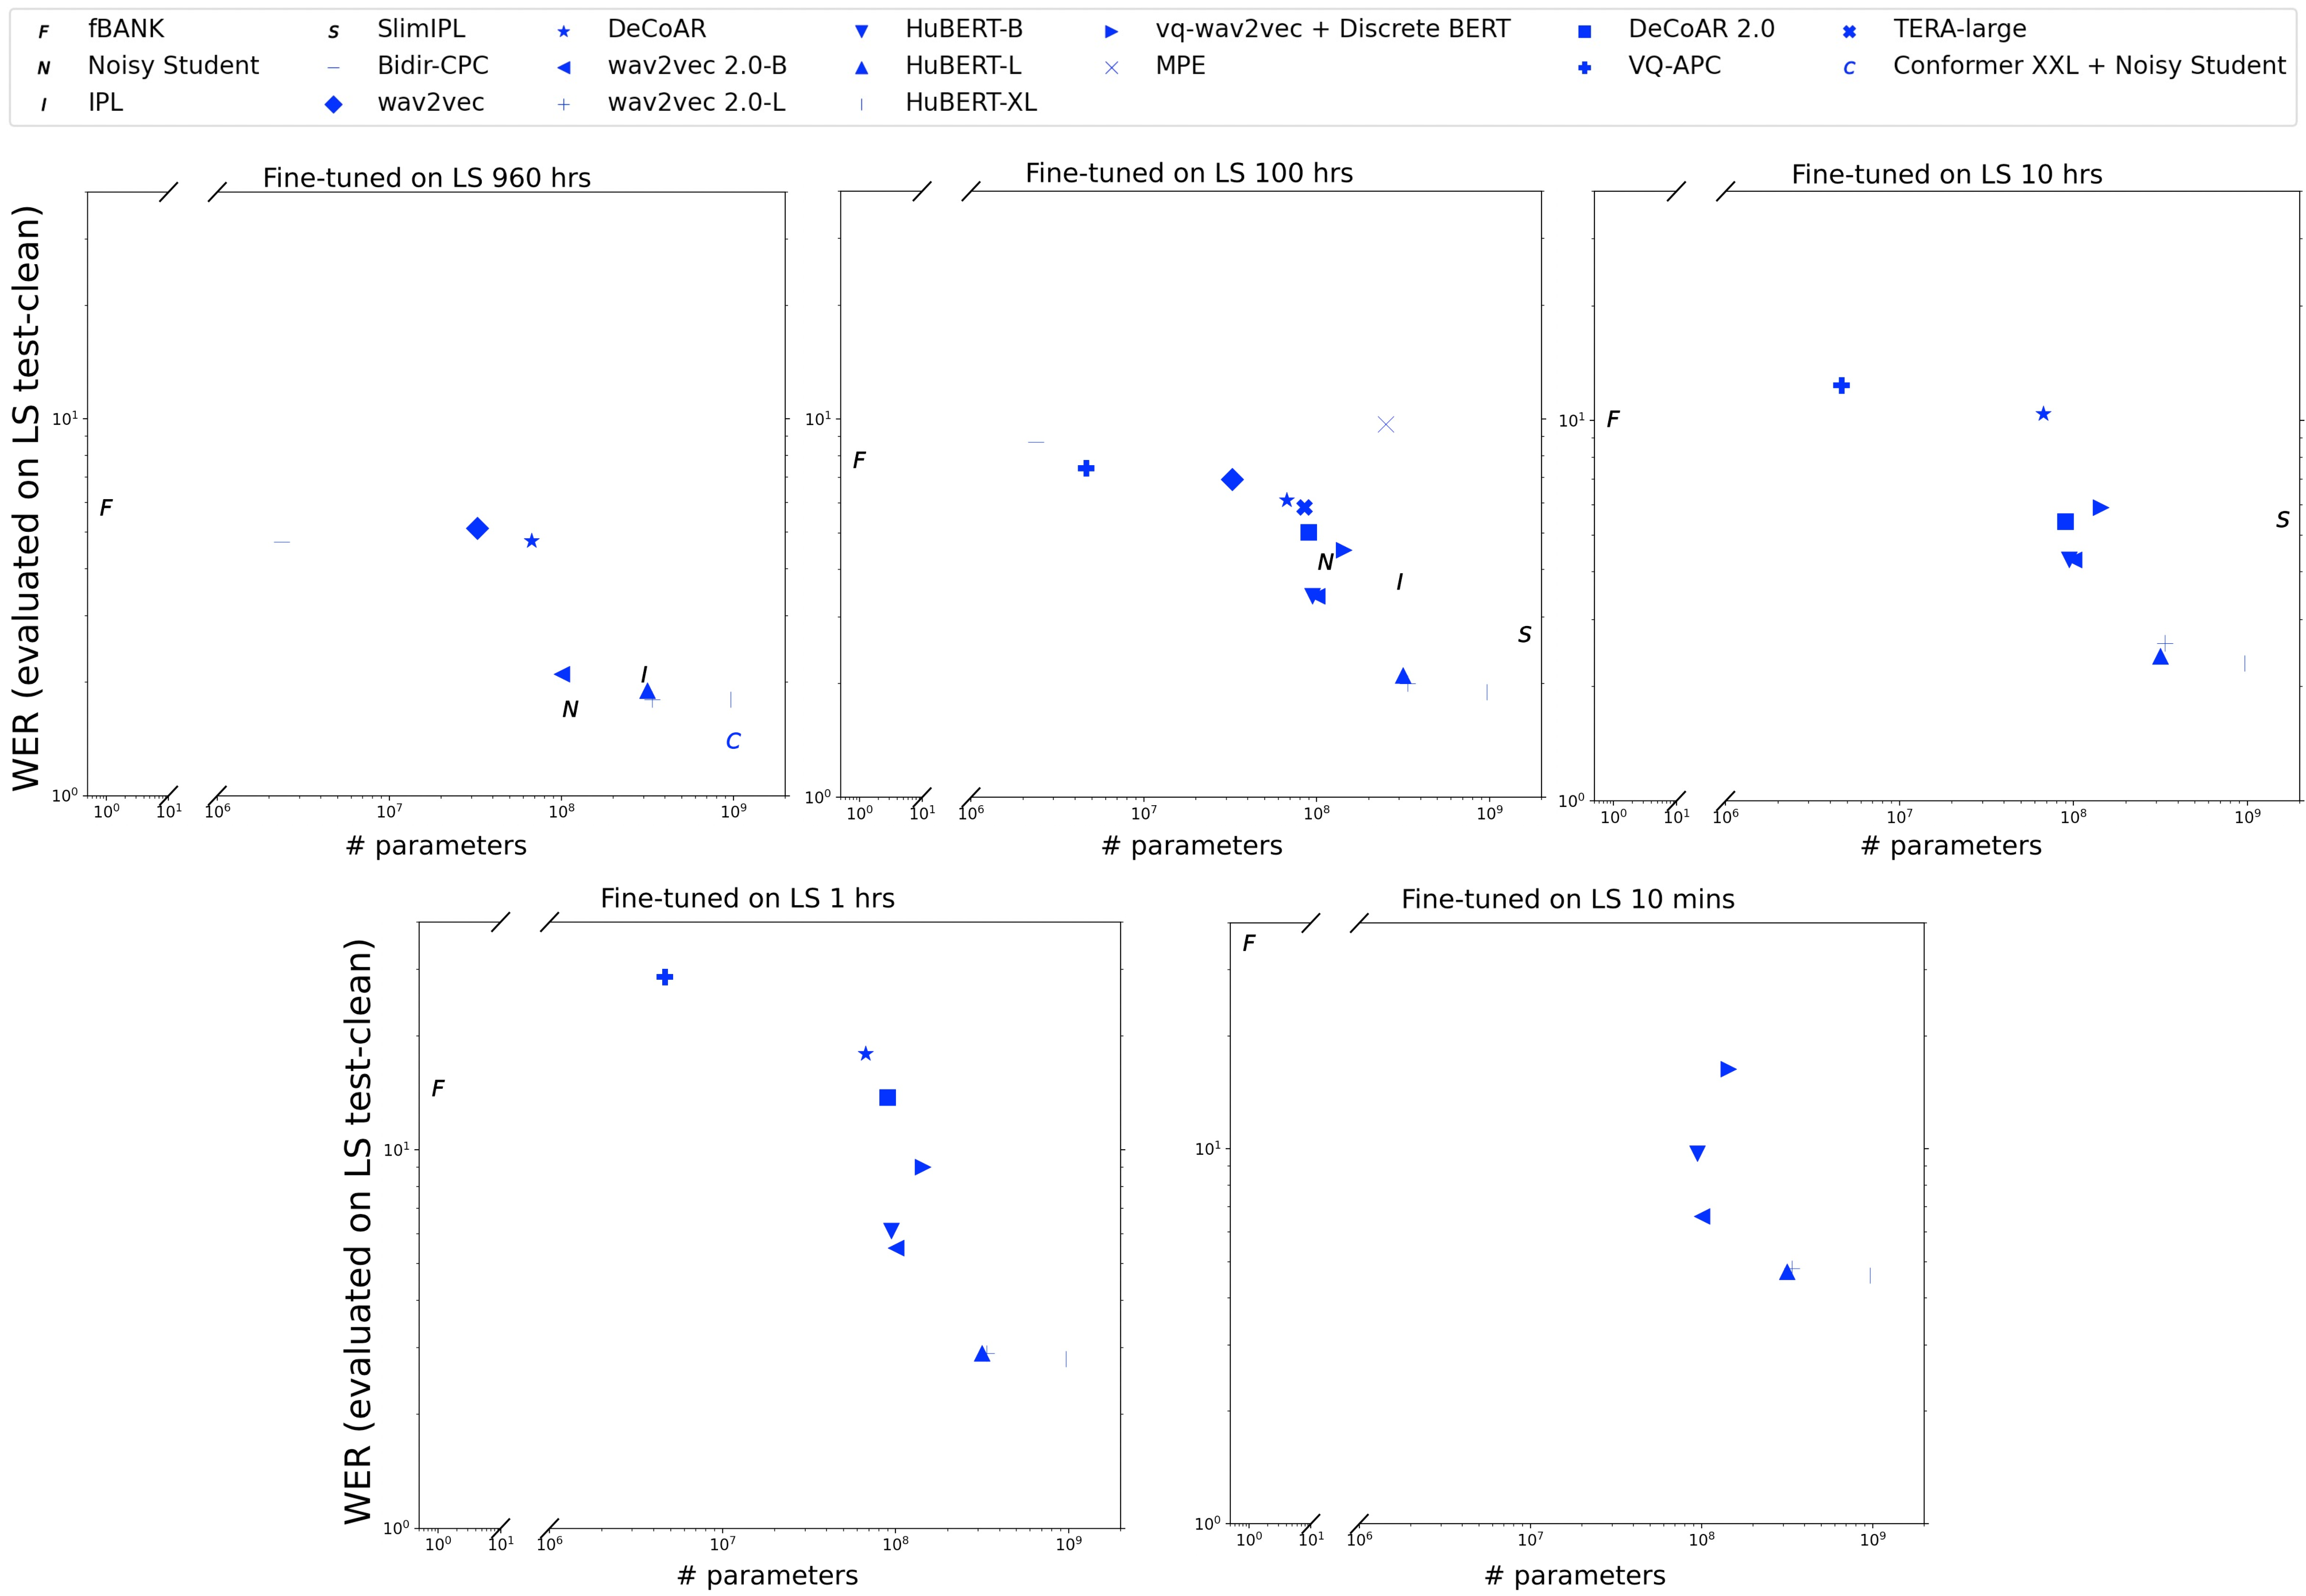
\includegraphics[width=0.9\textwidth]{paper_review/ls-test-clean-v2.pdf}
\caption[SSL performance for ASR evaluated on
LS \textit{test-clean}.]{SSL performance on ASR WER (vertical axis) evaluated with
LS \textit{test-clean} split. Techniques are sorted based on the number of
model parameters along the horizontal axis. Markers in blue correspond to models initialized with various SSL
techniques and then fine-tuned using 960, 100, 10, 1 hour(s), and 10 minutes
respectively. The 960-hour training set is the aggregation of
\textit{train-clean-100}, \textit{train-clean-360}, and
\textit{train-other-500} splits. The 100-, 10-, 1-hour, and 10-minute sets
leverage \textit{train-clean-100} or its sampling, except for Bidir-CPC, which
samples 10\% of the training examples from the entire 960-hour corpus. For simplicity,
several SSL techniques are appended with suffixes \textit{B}, \textit{L},
\textit{XL}, or \textit{XXL} indicating the \textit{Base}, \textit{Large},
\textit{X-Large}, or \textit{XX-Large} variants specified in the original
publication. We also compare with baselines including the log mel filterbank (fBANK) and semi-supervised, self-training
approaches (iterative pseudo labeling (IPL)~\cite{xu_iterative_2020}, 
slimIPL~\cite{likhomanenko_slimipl_2021}, noisy student~\cite{park_improved_2020}). These approaches are visualized in black. Also, note that the current state of the art---conformer XXL + noisy student~\cite{zhang_pushing_2020}---is a combination of self-training and SSL techniques. Given the
diversity of the listed methods in experiment settings (e.g., pre-training corpora
and objectives, whether a language model is used in decoding, whether model
parameters are frozen in fine-tuning), readers should be careful that the superiority
of methods cannot be decided only based on lower WER numbers.}
\label{fig:asr_result_no_limit}
\end{figure*}


\subsection{Benchmark results and discussion} \label{sec:benchmark} 
Given the diversity of datasets and downstream tasks used to evaluate SSL
techniques in the literature, it is infeasible to discuss all 
experiment settings in this survey. Hence, due to their wide adoption for
experiments conducted by studies in both SSL and the speech community in
general, we focus first on ASR on the LS dataset to understand the
efficacy of SSL. We examine SSL techniques which report ASR results on the LS
\textit{test-clean} split, and summarize the published WER in
\cref{fig:asr_result_no_limit}. The ASR models were obtained first by using
unlabeled speech to pre-train a model with each SSL technique. The model was
then fine-tuned on labeled data by utilizing a supervised training objective.
Respectively, 960, 100, 10, 1 hour(s), and 10 minutes of labeled LS training data
were used for fine-tuning, as indicated in different panels of
\cref{fig:asr_result_no_limit} (see
the caption of \cref{fig:asr_result_no_limit} for more details).
Semi-supervised methods such as self-training, where a model is first trained
on labeled data to annotate unlabeled speech, and then subsequently trained on
combined golden and self-annotated label-speech pairs, are gaining popularity
in the speech community and have yielded competitive results. For comparison, we also
show performance from such methods (iterative pseudo labeling 
(IPL)~\cite{xu_iterative_2020}, slimIPL~\cite{likhomanenko_slimipl_2021}, noisy 
student~\cite{park_improved_2020}), as well as the current state of the art---conformer XXL + noisy
student~\cite{zhang_pushing_2020}---which augments SSL with various advanced
techniques including self-training. Furthermore, we illustrate in the figure
the performance of a baseline system \cite{yang_superb_2021} based on log mel filterbank (fBANK), which is one of the most commonly used features designed by domain experts.
As observed in the figure, most SSL techniques outperform fBANK
features, and with the growing investment in model size, better performance is
achieved. The largest ones, such as wav2vec 2.0-L and HuBERT-L/XL, yield competitive results 
when the entire 960-hour of labeled data is used in
training/fine-tuning. The benefit of SSL, especially models with more parameters
like wav2vec 2.0 and HuBERT, becomes more evident when the labeling resources
become scarce. Compared to popular semi-supervised methods such as IPL,
slimIPL, and noisy student using 100 hours of labels, wav2vec~2.0 and HuBERT
achieve lower or competitive WERs with 1 hour or even 10 minutes of labeled
examples. The results are highly favorable for low-resource use cases, for instance when
expanding systems to new domains or languages for which large amounts of unlabeled
audio are available, since collecting labels for new conditions is often prohibitively
slow or costly.

In addition to the ASR task, where the current state of the art is achieved by a method
combining SSL pre-training and self-training 
techniques~\cite{zhang_pushing_2020}, SSL models are competitive in other tasks, including IC,
SID, ASV, and QbE. We summarize the performance of these models and previous
non-SSL methods in \cref{table:sota_performance}. The results suggest that the
benefit of SSL is generalizable among tasks that require encoding 
information such as content, speaker, and semantics. As SSL research
gains more attention, we expect that SSL pre-trained models will 
achieve state-of-the-art results on an increasing number of tasks.

\begin{table}[t!]
  \centering
  \footnotesize
  \caption{Tasks where the state of the art is models with SSL pre-training.}
  \label{table:sota_performance}
  \renewcommand*\arraystretch{1.2}
  \begin{tabular}{llllll}  
    \toprule
    Tasks & Dataset & non-SSL & SSL \\
    \midrule
    ASR (WER $\downarrow$) & LS test-clean/other & 2.1/4.0 \cite{xu_iterative_2020} & 1.4/2.6 \cite{zhang_pushing_2020} \\ \hline
    IC (Acc $\uparrow$) & FSC & 98.8 \cite{lugosch_speech_2019} & 99.3\cite{chen_unispeechsat_2021} \\ \hline
    SID (Acc $\uparrow$) & VoxCeleb1 & 94.8 \cite{hajibabaei_unified_2018} & 95.5 \cite{chen_wavlm_2021} \\ \hline
    ASV (EER $\downarrow$) & VoxCeleb1 & 3.1 \cite{hajavi_siamese_2021} & 2.4 \cite{wang_finetuned_2021} \\ \hline
    QbE (MTWV $\uparrow$) & QUESST (EN) & 10.6 \cite{rodriguez-fuentes_gttsehu_2014} & 11.2\cite{chen_unispeechsat_2021} \\
    \bottomrule
  \end{tabular}
\end{table}

Despite the obvious trend of increasing performance as more parameters and SSL
pre-training data are being used, numbers in \cref{fig:asr_result_no_limit} 
and \cref{table:sota_performance} are less comparable than might be expected.
The task performance is obtained from the original papers and is often
achieved with different downstream fine-tuning recipes, including various
language models (used in the ASR system), prediction heads (networks added to
SSL for downstream inference), or choices between fine-tuning the whole
networks or freezing the SSL encoders. For example, in the ASR task, HuBERT-L
and wav2vec~2.0-L leverage Transformer as their language model, while a 4-gram
language model trained on LS is used in DeCoAR~2.0. The lack of common and
established mechanisms to evaluate SSL techniques in downstream applications
makes it difficult to compare techniques fairly and understand their
capabilities. To address this challenge, there are increasing efforts to establish
benchmarks with shared downstream tasks, datasets, and downstream recipes. Such
efforts include SUPERB~\cite{yang_superb_2021}, 
LeBenchmark~\cite{evain_lebenchmark_2021}, ZeroSpeech~\cite{dunbar_zero_2020},
HEAR \cite{turian_hear_2022},
NOSS~\cite{shor_learning_2020}, and HARES~\cite{wang_learning_2021}. 

SUPERB~\cite{yang_superb_2021} is a benchmarking platform that allows the
SSL community to train, evaluate, and compare speech representations on
diverse downstream speech processing tasks, from acoustic and speaker identity
to paralinguistic and semantics. SUPERB consolidates downstream recipes to
focus on common and straightforward settings (e.g., prediction head
architectures, language models, hyperparameter spaces) to facilitate generalizable
and reproducible benchmarking of SSL techniques. SUPERB also encourages
researchers to innovate for efficient use of model parameters and computation
resources 
to democratize SSL beyond race among Big Tech.   % AMH: what does this mean?
LeBenchmark~\cite{evain_lebenchmark_2021} shares a vision similar to SUPERB and provides a
reproducible framework for assessing SSL in French with ASR, spoken language
understanding, speech translation, and emotion recognition. 
ZeroSpeech~\cite{dunbar_zero_2020} (described in more detail in \cref{zero_speech})
challenges the scientific community to build speech and language understanding
systems using zero expert resources 
for millions of users of ``low-resource" languages.
SSL techniques are also benchmarked with the ZeroSpeech 
challenge~\cite{tjandra_transformer_2020, vanniekerk_vectorquantized_2020}. Apart from the speech
community, researchers have also established HEAR (holistic evaluation of audio
representations) \cite{turian_hear_2022}, NOSS (non-semantic
speech benchmark)~\cite{shor_learning_2020}, and HARES (holistic audio
representation evaluation suite)~\cite{wang_learning_2021} to benchmark audio
representations. These efforts promote the creation of an audio embedding
that is as holistic as the human ear in interpreting speech, environmental
sound, and music. Given the significant need to understand and compare SSL techniques
fairly and comprehensively, we expect SSL benchmarking to remain an
active research area.

